\section{Method} \label{modeling.method}
CLIP stands for Contrastive Language-Image Pre-training, and it seeks to learn image representations that transfer to a wide range of downstream tasks such as image classification on datasets with a wide variety of source domains. To do so, it uses the task of pairing images with their corresponding captions for pre-training.   
% the Vision Transformer \citep{visiontransformer} as the image encoder; \texttt{B} stands for \textit{Base} model, and \texttt{32} stands for $32 \times 32$ input patch size. 
CLIP has two main parts: a text encoder and an image encoder, and both can be transformers. 
To model our dataset, we fine-tune the pre-trained \texttt{ViT-B/32} CLIP model using the \texttt{Python} \texttt{clip} package. 

In this section, we will first introduce the details of the CLIP contrastive objective (Section \ref{clip.objective}). We will then introduce the pre-trained transformer-based text and image encoders in Section \ref{clip.text.encoder} and \ref{clip.image.encoder}, respectively. Lastly, in Section \ref{clip.finetune}, we explain how we preprocess sketches and texts for fine-tuning and how we use CLIP to perform the task in Section \ref{modeling.task.def}.

\subsection{Contrastive Objective} \label{clip.objective}

\begin{figure*}[!htb]
\centering
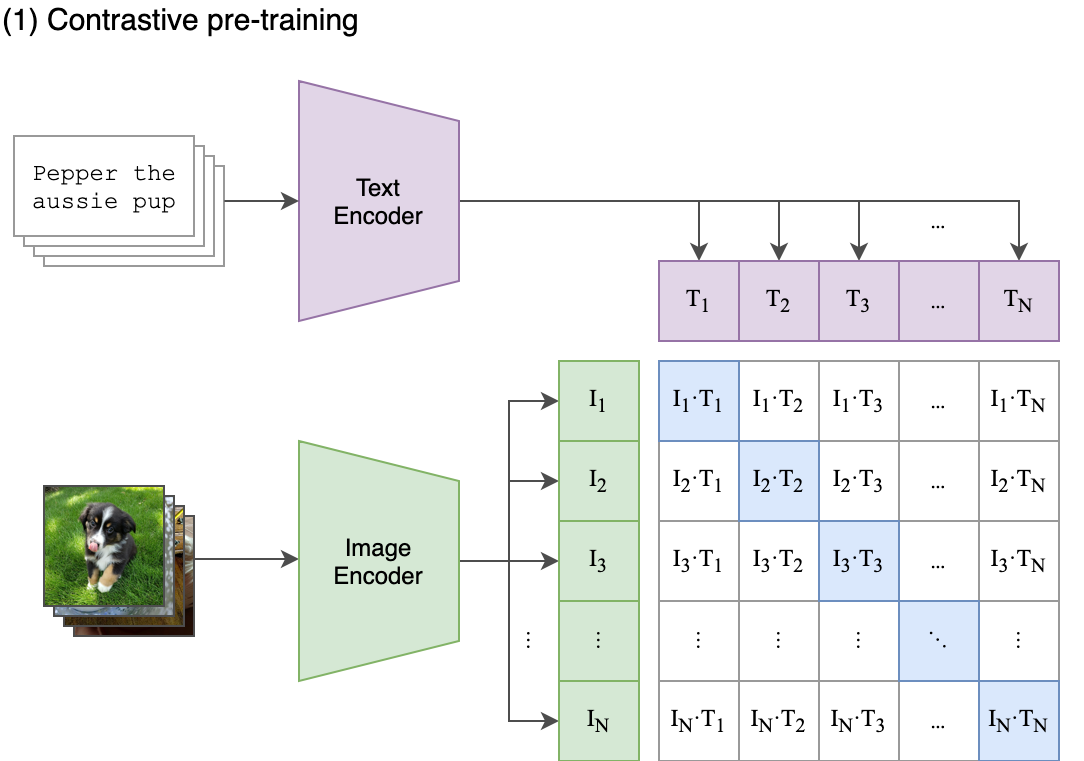
\includegraphics[width=0.7\linewidth]{modeling/CLIP.png}  
\caption{CLIP uses contrastive instead of generative objective for pre-training to learn joint vision-language embeddings. This image is taken from Figure 1 in the original CLIP paper \citep{CLIPpaper}. Each grid contains the dot-product of normalized image,text features.}
\label{modeling.clip.pretrainingobj}
\end{figure*}

Pre-training on an enormous amount of image-caption data with a contrastive objective, CLIP is able to learn robust vision-language joint embedding that allows it to perform on par with state-of-the-art (SOTA) models learnt with supervised objectives \citep{CLIPpaper}.  
% It is difficult to predict the exact captions for an image, since there is usually a wide variety of text descriptions co-occuring with images, so instead CLIP turns to contrastive objectives and solves the problem of determining which text and image should be matched together. 
During pre-training, for a batch of $N$ (text, image) pairs, CLIP obtains $N$ image features, $I_1,\dots,I_N$, and $N$ text features, $T_1,\dots,T_N$, from the encoders. 
It then calculates dot-product between each pair of normalized vectors, where there are $N \times N$ possible pairing in total, as shown in the grid in Figure \ref{modeling.clip.pretrainingobj}.
This grid is a logit matrix $X$ of dimension $N\times N$ and $X_{ij} = I_i \cdot T_j$. 
If we normalize the $i$-th row ($i \in [N]$) through softmax ($\frac{\exp\{ {X}_{i,i} \}}{ \sum_{j=1}^N \exp\{ {X}_{i,j}\}}$), we obtain a distribution over the captions representing the likelihood of pairing the $j$-th caption with the $i$-th image. 
Similarly, normalizing the $j$-th column through softmax gives a distribution over all the images of how likely an image pairs with the $j$-th caption. 

As explained in \cite{CLIPpaper}, we can treat each batch as containing $N$ visual concepts expressed through language.
By normalizing the rows and columns into distributions, we perform classification over the $N$ captions for the images and classification over the $N$ images for the captions.  
Moreover, we know that the ground-truth is pairing the $i$-th image with the $i$-th caption.   
Therefore, for classification over captions, we have the ground-truth vector $Y_I$; for classification over images, we have the ground-truth vector $Y_T$, and we know: 
$$Y_I = Y_T = \begin{bmatrix}1 & 2 & \cdots & N \end{bmatrix}^T $$ 
Similar to standard multi-class classification, we can use cross-entropy loss as our objective function. The loss $L_I(X, Y)$ of selecting the correct caption for each image:
\begin{equation} \label{cliploss.image}
\begin{split}
    L_I(X, Y) = \dfrac{1}{N} \sum_{i=1}^N -\log\frac{\exp\{ {X}_{i,i} \}}{ \sum_{j=1}^N \exp\{ {X}_{i,j} \} }
\end{split}
\end{equation}
The loss $L_T(X, Y)$ of selecting the correct image for each caption:
\begin{equation} \label{cliploss.text}
\begin{split}
    L_T(X, Y) = \dfrac{1}{N} \sum_{j=1}^N -\log\frac{\exp\{ {X}_{j,j} \}}{ \sum_{i=1}^N \exp\{ {X}_{i,j} \} }
\end{split}
\end{equation}
The final loss is defined as:
\begin{equation} \label{cliploss.all}
\begin{split}
    L = \dfrac{1}{2} (L_I(X, Y) + L_T(X, Y))
\end{split}
\end{equation}

In order to minimize the cross-entropy loss, the model has to increase the logits on the diagonal of $X$, which means that it has to learn an embedding space where the feature vectors of the $i$-th image and the $i$-th caption are similar and the feature vectors of the other pairs are far apart. The term \textit{contrastive} in the title of CLIP comes from this objective to pull together the real pair in the joint embedding space.    

%%%%%%%%%%%%%%%%%%%%%%%%%%%%%%%%%%%%%%%%
%%%%%%%%%%%%%%%%%%%%%%%%%%%%%%%%%%%%%%%%
%%%%%%%%%%%%%%%%%%%%%%%%%%%%%%%%%%%%%%%%
%%%%%%%%%%%%%%%%%%%%%%%%%%%%%%%%%%%%%%%%
%%%%%%%%%%%%%%%%%%%%%%%%%%%%%%%%%%%%%%%%
%%%%%%%%%%%%%%%%%%%%%%%%%%%%%%%%%%%%%%%%
%%%%%%%%%%%%%%%%%%%%%%%%%%%%%%%%%%%%%%%%
%%%%%%%%%%%%%%%%%%%%%%%%%%%%%%%%%%%%%%%%
%%%%%%%%%%%%%%%%%%%%%%%%%%%%%%%%%%%%%%%%
%%%%%%%%%%%%%%%%%%%%%%%%%%%%%%%%%%%%%%%%
%%%%%%%%%%%%%%%%%%%%%%%%%%%%%%%%%%%%%%%%
%%%%%%%%%%%%%%%%%%%%%%%%%%%%%%%%%%%%%%%%
%%%%%%%%%%%%%%%%%%%%%%%%%%%%%%%%%%%%%%%%
%%%%%%%%%%%%%%%%%%%%%%%%%%%%%%%%%%%%%%%%
%%%%%%%%%%%%%%%%%%%%%%%%%%%%%%%%%%%%%%%%
%%%%%%%%%%%%%%%%%%%%%%%%%%%%%%%%%%%%%%%%
%%%%%%%%%%%%%%%%%%%%%%%%%%%%%%%%%%%%%%%%
%%%%%%%%%%%%%%%%%%%%%%%%%%%%%%%%%%%%%%%%

\subsection{Text Encoder} \label{clip.text.encoder}

\subsubsection*{Overview of Transformer Architecture}
% \paragraph{Transformer: Attention is All You Need}
\begin{figure*}[!htb]
\begin{subfigure}{0.5\textwidth}
    \centering
    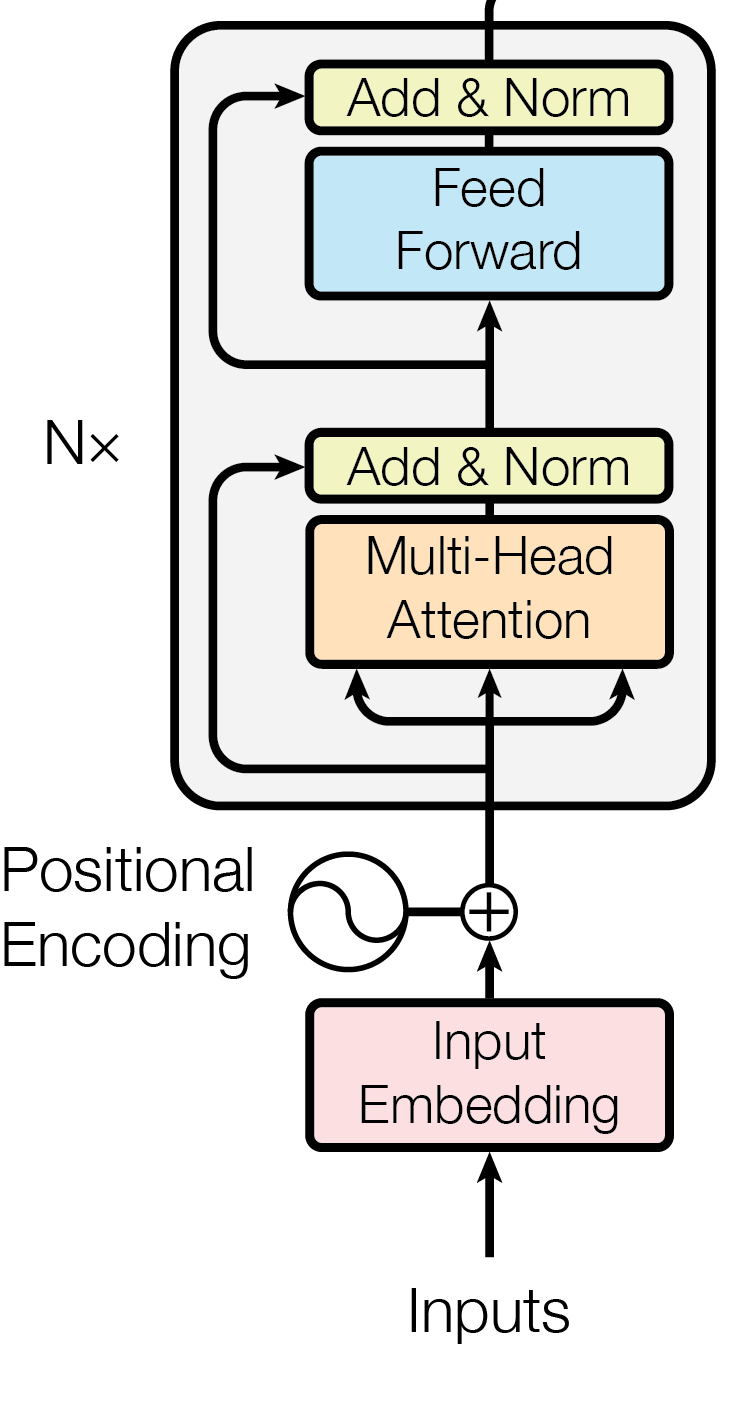
\includegraphics[width=0.5\linewidth]{modeling/transformer.png}  
    \caption{Encoder architecture used in original Transformer paper; the figure is taken from Figure 1 in \cite{attentionAllYouNeed}.}
    \label{modeling.transformer.origEncoder}
\end{subfigure}
\hspace{5mm}
\begin{subfigure}{0.5\textwidth}
    \centering
    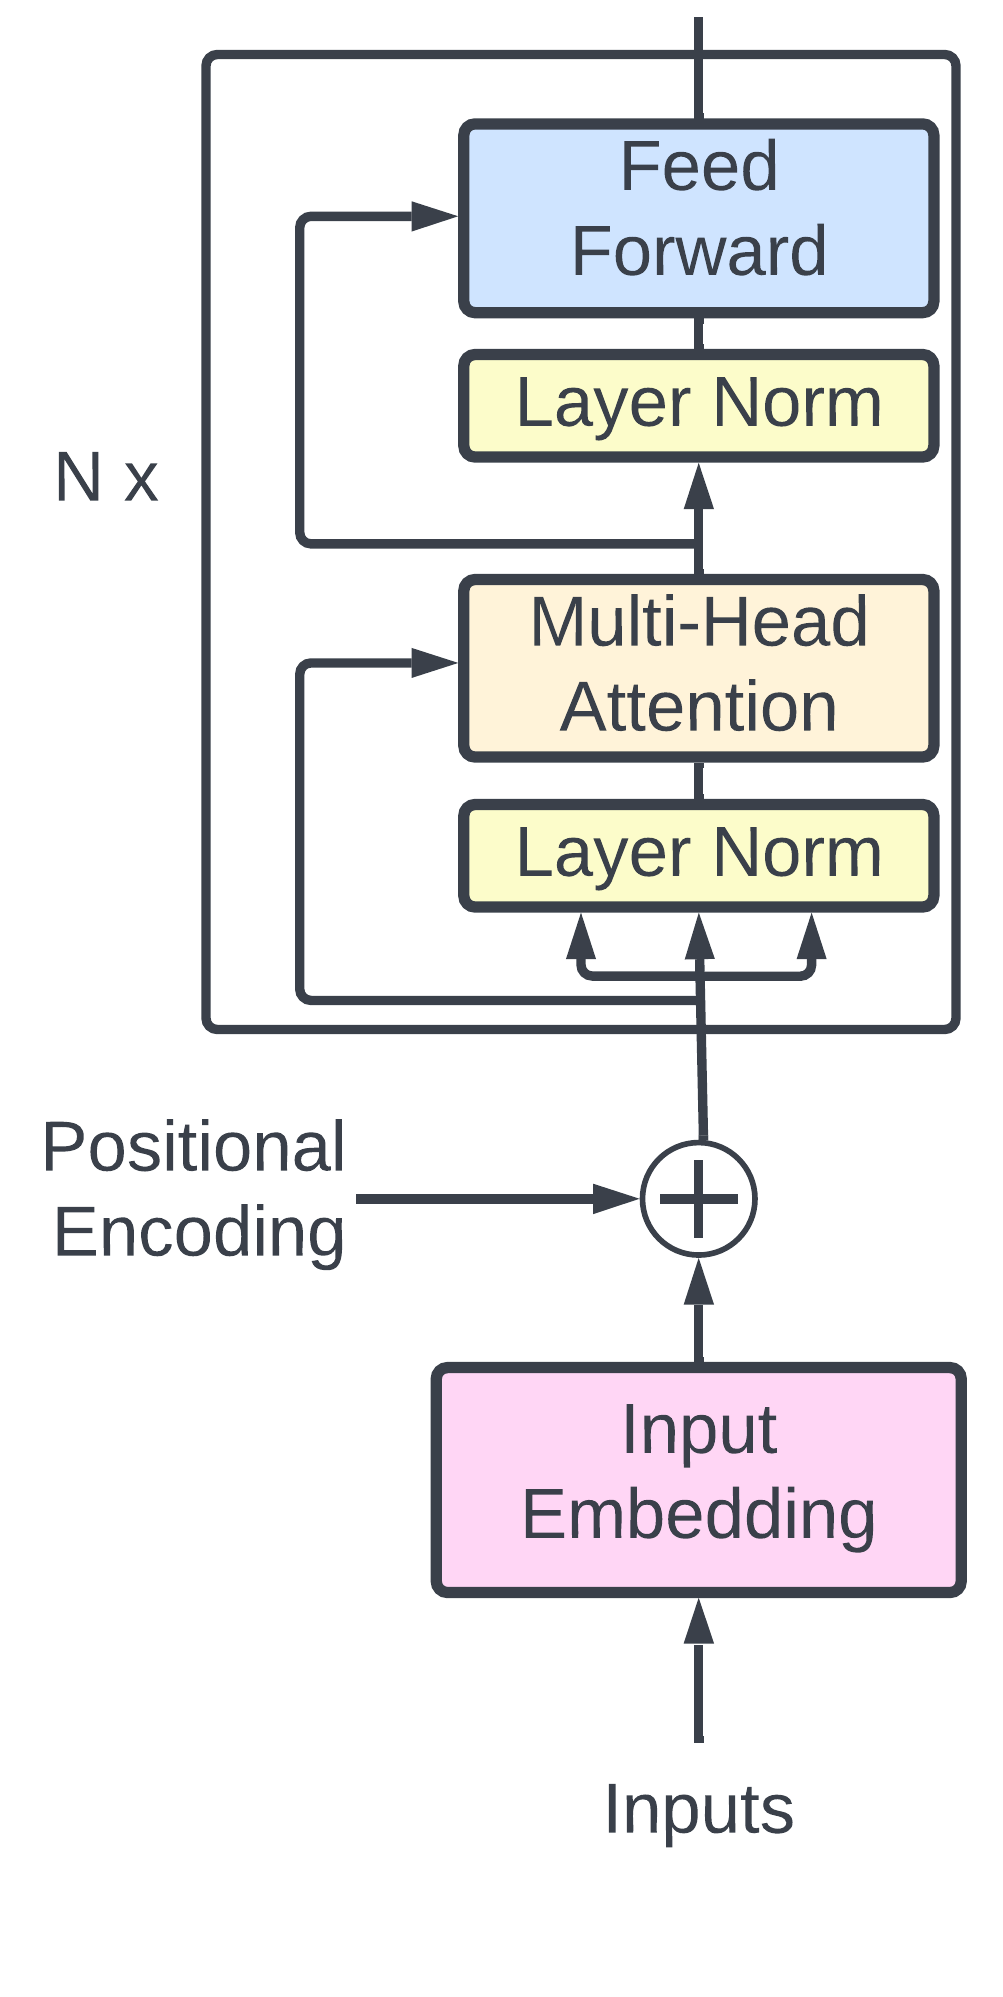
\includegraphics[width=0.5\linewidth]{modeling/clip_text_transformer.png}   
    \caption{Encoder architecture of CLIP \citep{CLIPpaper}.}
    \label{modeling.attention.clipEncoder}
\end{subfigure}
\caption{Text encoder architecture: the text encoder is a transformer with stacked layers of self-attention and feed-forward network sublayers. The main implementation difference between the original Transformer (on the left) and the transformer implemented by CLIP is the placement of layer normalization.}
\label{modeling.transformer}
\end{figure*}

The text encoder of CLIP is based on the transformer architecture introduced in \citet{attentionAllYouNeed}. Transformer relies only on self-attention mechanism to compute a representation for the input sequence. In this way, it alleviates the computation inefficiency and difficulty capturing long-range dependencies witnessed in recurrent layers.  

Figure \ref{modeling.transformer.origEncoder} and \ref{modeling.attention} are the same figures used in \cite{attentionAllYouNeed} to illustrate the transformer architecture. In Figure \ref{modeling.transformer.origEncoder}, \cite{attentionAllYouNeed} gives an overview of the encoder architecture. Firstly, tokenized texts go through an embedding layer; the input embeddings are summed with learned position embeddings that inject information on order of the sequence. 
% and incorporated modification suggested in \citet{Radford2019LanguageMA}
The input is computed using Byte Pair Encoding (BPE) with a $49,152$ vocabulary. As explained in the GPT-2 paper, BPE, a sub-word tokenization scheme, strikes a good balance between word-level and character-level word embeddings, since one works well with common words and the other with rare sequences \citep{Radford2019LanguageMA}.

\begin{figure*}[!htb]
\begin{subfigure}{0.5\textwidth}
\centering
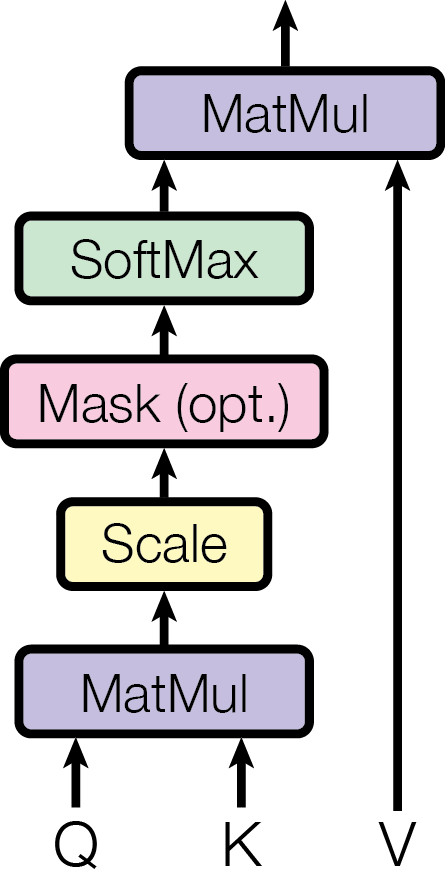
\includegraphics[width=.3\linewidth]{modeling/selfAttention.png}  
\end{subfigure}
\begin{subfigure}{0.5\textwidth}
\centering
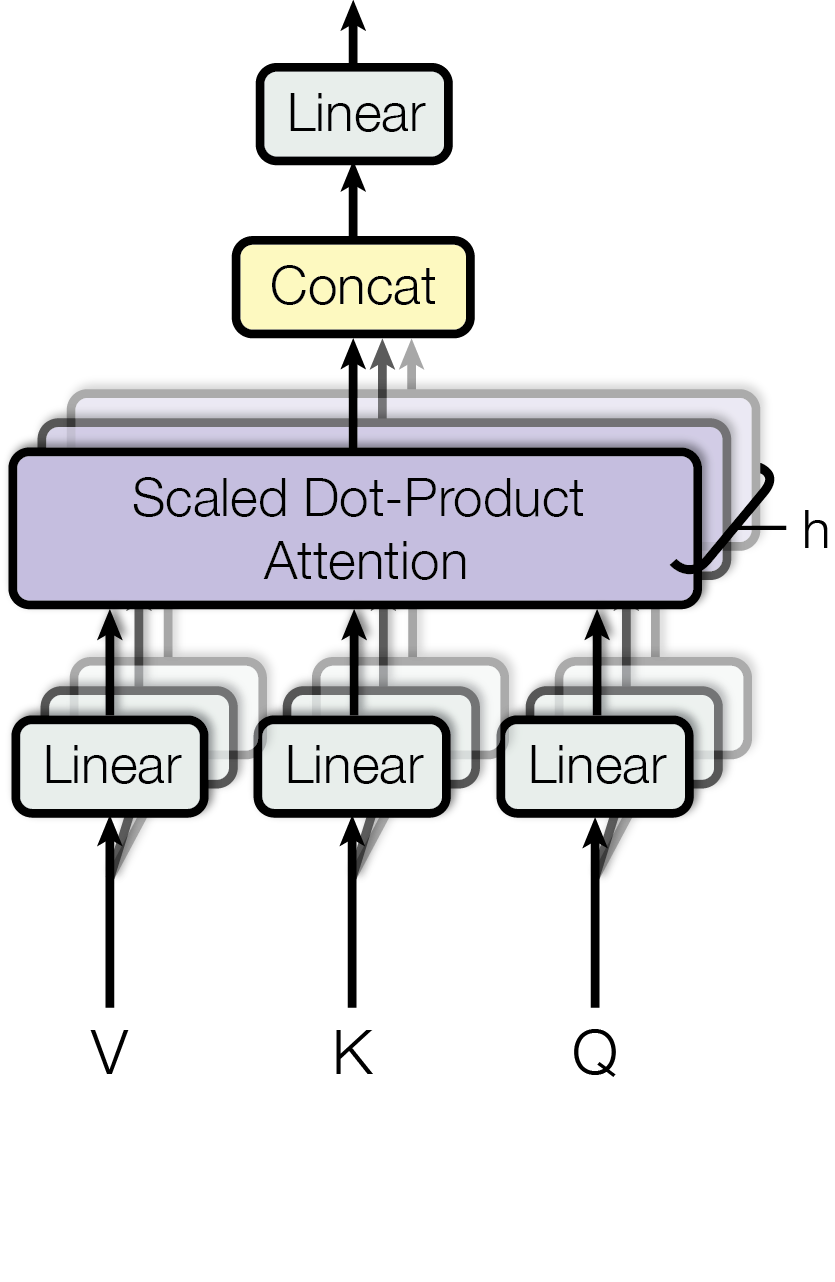
\includegraphics[width=.5\linewidth]{modeling/multiHeadAttention.png}  
\end{subfigure}
\caption{An illustration of the scaled dot-product attention on the left; on the right, an illustration of the multi-head self-attention mechanism (MSA) used in every layer of the transformer. Both figures are from the original Transformer paper \citep{attentionAllYouNeed}.}
\label{modeling.attention}
\end{figure*}

Next, the input is passed through stacked layers multi-head self-attention (MSA) mechanism followed by point-wise feed-forward networks (FFN). 
In the version of CLIP that we use, the text encoder is a 12-layer transformer, and the model dimenison is $512$, $d_{model} = 512$, meaning that output of the initial embedding layers, MSA, FFN all have dimension $512$.  

Compare to the formulation $LayerNorm(x + Sublayer(x))$ used in \cite{attentionAllYouNeed} (Figure \ref{modeling.transformer.origEncoder}), the CLIP text encoder uses $x + Sublayer(LayerNorm(x))$ (Figure \ref{modeling.attention.clipEncoder}), where $Sublayer$ refers to either MSA or FFN. Each layer still contains residual connection and layer normalization, but the order is switched between \cite{attentionAllYouNeed} and \cite{CLIPpaper}. 

\subsubsection*{Multi-Head Self-Attention}
As illustrated in Figure \ref{modeling.attention}, given query, key, value matricies $Q,K,V$ (in our case, all three matrices equal to the input text embeddings), transformer uses different linear projections to create multi-head attention, and \citet{attentionAllYouNeed} explains the benefit of multi-head attention as allowing the model to attend simultaneously to multiple representation subspaces of the input.      

\begin{equation} \label{mha}
\begin{split}
    MultiHead(Q,K,V) & = Concat({head}_1,\dots,{head}_h)W^O \\
    {head}_i & = Attention(QW_i^{Q}, KW_i^{K}, VW_i^{V}) \\
    Attention(Q,K,V) & = softmax(\dfrac{QK^T}{\sqrt{d_k}})V 
\end{split}
\end{equation}

$\text{ViT-B}/32$ uses a version with $h = 8$ attention heads, so $W_i^{Q}, W_i^{K} \in \mathbb{R}^{d_{model} \times d_k}$ and $W_i^{V} \in \mathbb{R}^{d_{model} \times d_v}$, where $d_k = d_v = \dfrac{d_{model}}{h} = \frac{512}{8} = 64$. 
At the end of the multi-head attention mechanism, the weighted combination of values from each head is concatenated together and passed through a linear layer, represented here as $W^O \in \mathbb{R}^{(d_v \times h) \times d_v}$. 
CLIP uses the ``Scaled Dot-Product Attention'' in \cite{attentionAllYouNeed}, illustrated in details in Figure \ref{modeling.attention}. The dot products between query and key determine the weights that are used to sum the values; in this way, we have a contextualized representation; compared to convolutions that use static kernels, attention weights are dynamic.   

%%%%%%%%%%%%%%%%%%%%%%%%%%%%%%%%%%%%%%%%
%%%%%%%%%%%%%%%%%%%%%%%%%%%%%%%%%%%%%%%%
%%%%%%%%%%%%%%%%%%%%%%%%%%%%%%%%%%%%%%%%
%%%%%%%%%%%%%%%%%%%%%%%%%%%%%%%%%%%%%%%%
%%%%%%%%%%%%%%%%%%%%%%%%%%%%%%%%%%%%%%%%
%%%%%%%%%%%%%%%%%%%%%%%%%%%%%%%%%%%%%%%%
%%%%%%%%%%%%%%%%%%%%%%%%%%%%%%%%%%%%%%%%
%%%%%%%%%%%%%%%%%%%%%%%%%%%%%%%%%%%%%%%%
%%%%%%%%%%%%%%%%%%%%%%%%%%%%%%%%%%%%%%%%
%%%%%%%%%%%%%%%%%%%%%%%%%%%%%%%%%%%%%%%%
%%%%%%%%%%%%%%%%%%%%%%%%%%%%%%%%%%%%%%%%
%%%%%%%%%%%%%%%%%%%%%%%%%%%%%%%%%%%%%%%%
%%%%%%%%%%%%%%%%%%%%%%%%%%%%%%%%%%%%%%%%
%%%%%%%%%%%%%%%%%%%%%%%%%%%%%%%%%%%%%%%%
%%%%%%%%%%%%%%%%%%%%%%%%%%%%%%%%%%%%%%%%
%%%%%%%%%%%%%%%%%%%%%%%%%%%%%%%%%%%%%%%%
%%%%%%%%%%%%%%%%%%%%%%%%%%%%%%%%%%%%%%%%
%%%%%%%%%%%%%%%%%%%%%%%%%%%%%%%%%%%%%%%%

\subsection{Image Encoder} \label{clip.image.encoder}
\begin{figure*}[!htb]
\centering
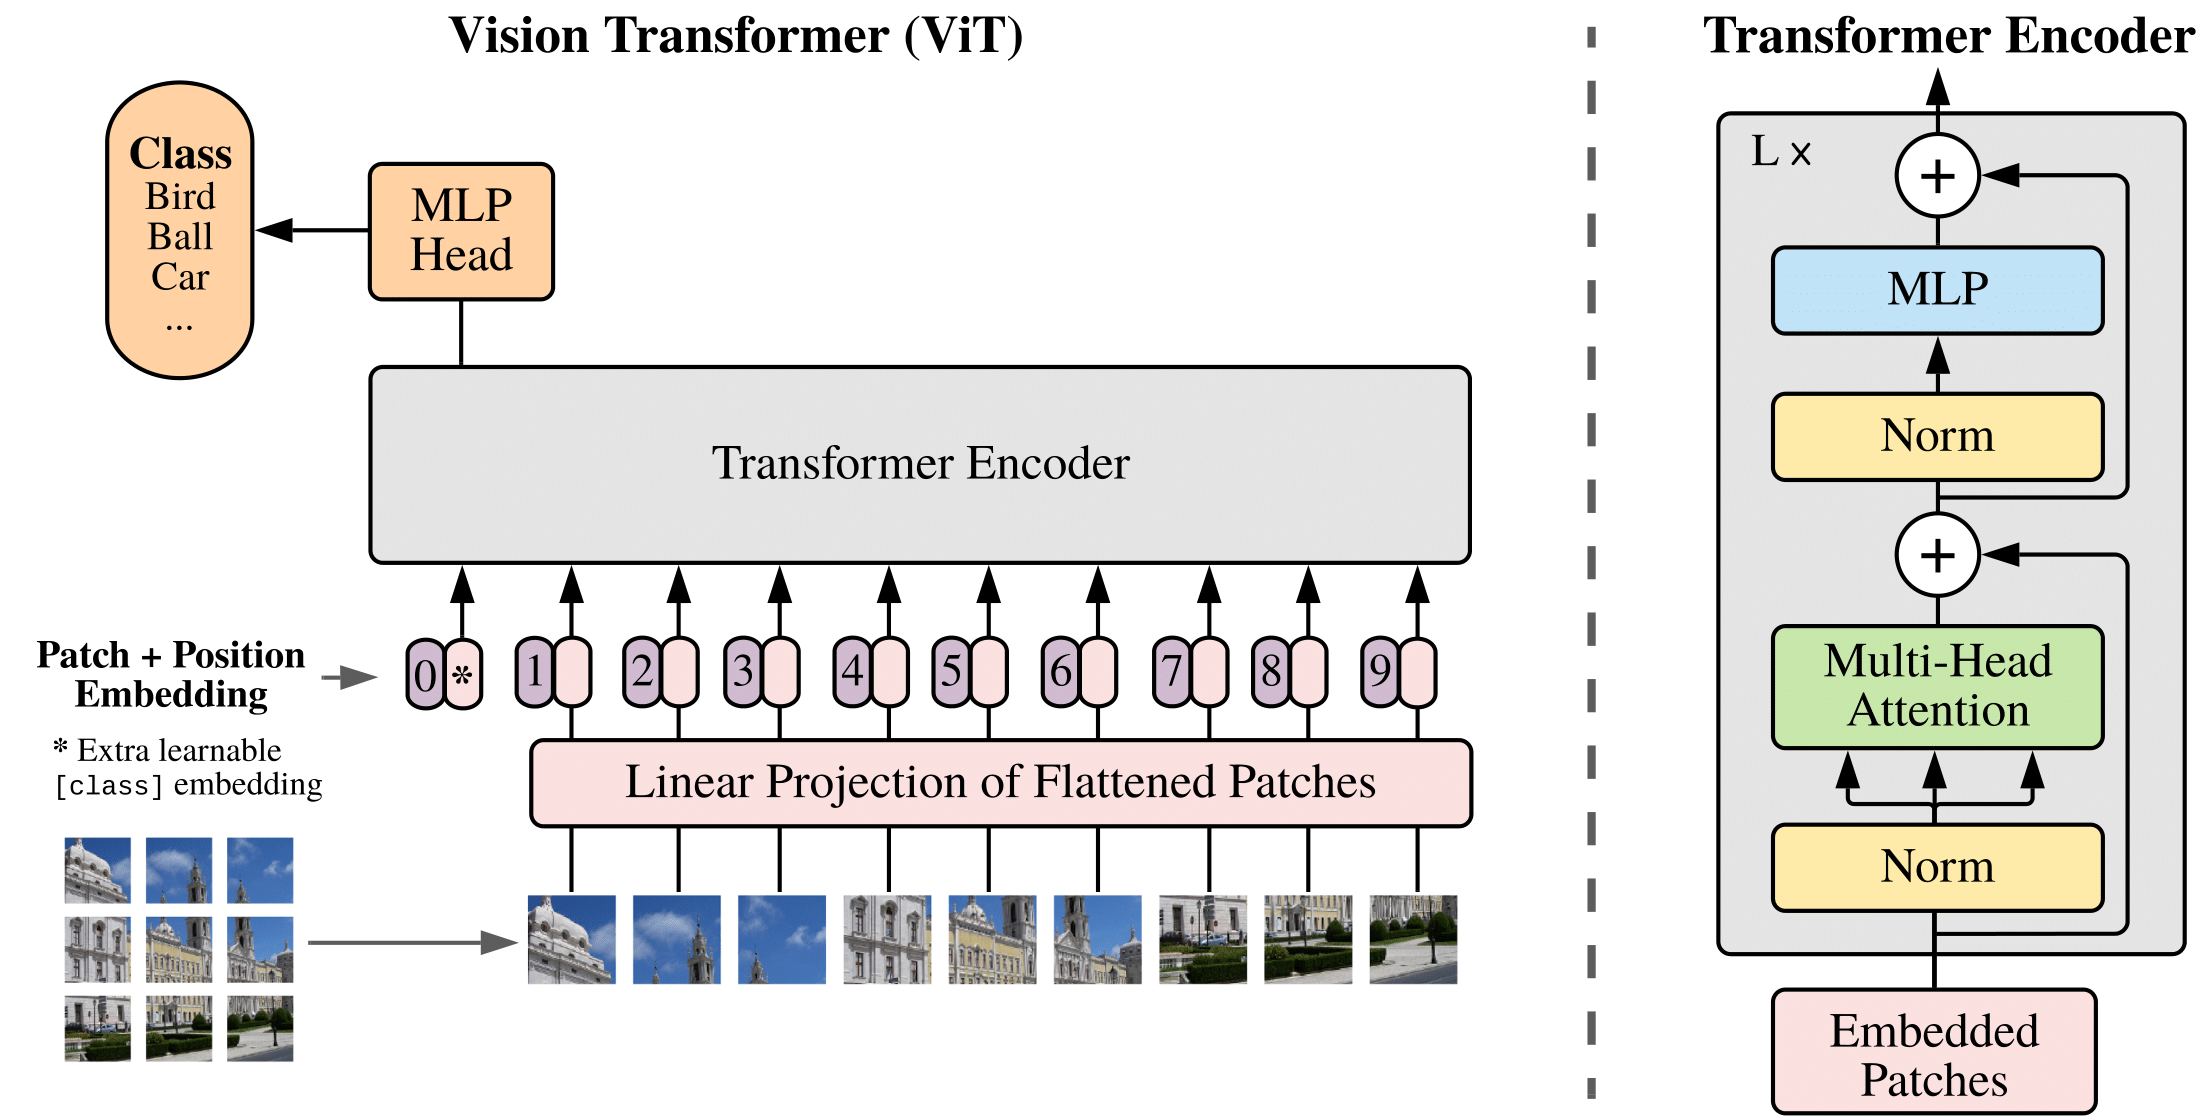
\includegraphics[width=0.7\linewidth]{modeling/visionTransformer.png}  
\caption{Vision Transformer (ViT) architecture \citep{ViT}.}
\label{modeling.visionTransformer}
\end{figure*}

The image encoder of CLIP uses Vision Transformer (ViT) introduced in \cite{ViT}. The architecture of ViT is based on the original transformer introduced in \cite{attentionAllYouNeed}. 
In order to reuse the transformer model, ViT needs to first turn an image of size $H\times W \times C$, ($H$, $W$, $C$ stands for image height, width, channel size, respectively), into a sequence of ``tokens'', similar to the text input.  
To do so, \cite{ViT} reshapes the image to size $N \times (P^2 \cdot C)$, where $N$ is the number of patches and $P$ the patch size; the reshaped image can be seen as a sequence of $N$ image tokens, each having a dimension of $P^2 \cdot C$. Each image token is then passed through a linear layer to be mapped to dimension $D$, similar to the model dimension $d_{model}$ earlier. 

In the version of CLIP that we used, all input images have dimension $224\times 224$, the patch size $P = 32$, and the output of the initial embedding layers, MSA, FFN all have dimension $768$ ($D = 768$). 
As explained in \cite{ViT}, before passing into the transformer, we also need to prepend a \texttt{[class]} token at the front the sequence, whose embedding at the last layer of the transformer will be used as the representation for the entire image. In this way, each image is represented as a sequence of $7\times 7 + 1 = 50$ tokens, illustrated as purple boxes in Figure \ref{modeling.visionTransformer}. The pink boxes that are right next to the patch embeddings represent position embeddings, with a similar function to encoder sequence order information as in the text transformer. 
For the CLIP image encoder, layer normalization is applied to the input before passing into the transformer and to the output at the last layer.
 

%%%%%%%%%%%%%%%%%%%%%%%%%%%%%%%%%%%%%%%%
%~~~~~~~~~~~~~~~~~~~~~~~~~~~~~~~~~~~~~~%
%~~~~~~~~~~~~~~~~~~~~~~~~~~~~~~~~~~~~~~%
%~~~~~~~~~~~~~~~~~~~~~~~~~~~~~~~~~~~~~~%
%~~~~~~~~~~~~~~~~~~~~~~~~~~~~~~~~~~~~~~%
%~~~~~~~~~~~~~~~~~~~~~~~~~~~~~~~~~~~~~~%
%~~~~~~~~~~~~~~~~~~~~~~~~~~~~~~~~~~~~~~%
%~~~~~~~~~~~~~~~~~~~~~~~~~~~~~~~~~~~~~~%
%~~~~~~~~~~~~~~~~~~~~~~~~~~~~~~~~~~~~~~%
%~~~~~~~~~~~~~~~~~~~~~~~~~~~~~~~~~~~~~~%
%~~~~~~~~~~~~~~~~~~~~~~~~~~~~~~~~~~~~~~%
%~~~~~~~~~~~~~~~~~~~~~~~~~~~~~~~~~~~~~~%
%~~~~~~~~~~~~~~~~~~~~~~~~~~~~~~~~~~~~~~%
%~~~~~~~~~~~~~~~~~~~~~~~~~~~~~~~~~~~~~~%
%~~~~~~~~~~~~~~~~~~~~~~~~~~~~~~~~~~~~~~%
%~~~~~~~~~~~~~~~~~~~~~~~~~~~~~~~~~~~~~~%
%~~~~~~~~~~~~~~~~~~~~~~~~~~~~~~~~~~~~~~%
%~~~~~~~~~~~~~~~~~~~~~~~~~~~~~~~~~~~~~~%
%~~~~~~~~~~~~~~~~~~~~~~~~~~~~~~~~~~~~~~%
%~~~~~~~~~~~~~~~~~~~~~~~~~~~~~~~~~~~~~~%
%~~~~~~~~~~~~~~~~~~~~~~~~~~~~~~~~~~~~~~%
%~~~~~~~~~~~~~~~~~~~~~~~~~~~~~~~~~~~~~~%
%%%%%%%%%%%%%%%%%%%%%%%%%%%%%%%%%%%%%%%%

\subsection{Fine-Tuning CLIP} \label{clip.finetune}


We fine-tune CLIP with our dataset containing (sketch, part description) pairs. Our sketches come from the QuickDraw dataset \citep{ha2017neural}, and the semantic part annotations come from the SPG dataset \citep{spg_paper}. We collected text descriptions from turkers for every part in face and angel sketches; details of the data collection process are in Section \ref{datav2}, and we summarize the dataset in Section \ref{datasummary}.  
% We will present how we pre-process the image data to fine-tune CLIP (\ref{sketch.preprocess}). Through data collection (Chapter \ref{dataChapter}), we obtained text descriptions of semantic parts provided by SPG, and we present how they are cleaned-up for fine-tuning in (\ref{text.preprocess}).   

\subsubsection*{Sketch Preprocessing} \label{sketch.preprocess}
The QuickDraw sketches are stored in vector format: each sketch is composed of a sequence of $n$ strokes $S_i, i \in [n]$, and each stroke $S_i$ is a sequence of vectors $(\delta x,\delta y, p, l)$. 
$\delta x$ and $\delta y$ are changes in the $x,y$ coordinates with respect to the previous point; for the first point, its coordinate is with respect to the point $(25,25)$. 
All points are assumed to be drawn on a $256 \times 256$ canvas. 
$p=1$ if the point is the last point in the current stroke, and $p=0$ otherwise. 
The SPG dataset provides annotation for semantic segmentation of the sketches \citep{spg_paper}, and $l$ is an integer representing which semantic part the current point belongs to. For face sketches, the parts can be \textit{eyes}, \textit{nose}, \textit{mouth}, \textit{hair}, or \textit{outline of face}; for angel sketches, the parts can be \textit{halo}, \textit{eyes}, \textit{nose}, \textit{mouth}, \textit{body}, \textit{outline of face}, or \textit{wings}.
% For angels, $l = 0$ if the point is part of the eyes.   
% $$ for \textit{halo}, \textit{eyes}, \textit{nose}, \textit{mouth}, \textit{body}, \textit{outline of face}, \textit{wings}; for face, $\texttt{[PART NAME]}$ is one of \textit{eyes}, \textit{nose}, \textit{mouth}, \textit{hair}, \textit{outline of face}. 

During training, we render the sketches from the vector format into PNG images using the python package \texttt{cairocffi}. To augment the data, we did: (1) sample stroke width uniformly from the range $[2.5,12.5]$; (2) rotate the sketches randomly by sampling an angle from the range $[-\frac{\pi}{4}, \frac{\pi}{4}]$; (3) scale the sketches with the scale factor sampled from the range $[0.75, 1.25]$; (4) translate the strokes vertically or horizontally with $0.15$ as the maximum absolute fraction translation.   
% 'rotate' : [-1/4*180, 1/4*180],
% 'trans' : [0.15, 0.15],
% 'scale' : [0.75, 1.25],
% 'open_clip' : False,
% 'adamw' : False,
% 'no_image_augment' : False,
% We obtained the rendered sketches by using \texttt{Pycairo}, which is a Python module providing bindings for the cairo graphics library. We use a line width of $5$. After rendering, we manually examined the sketches and filter out face sketches that do not have a pair of eyes, a mouth and the face outline; we also filter out angel sketches that are incomplete or have all the parts merged together, possibly due to collection errors in SPG.  

\subsubsection*{Text Preprocessing} \label{text.preprocess}
We used the spaCy package to preprocess the text \citep{spacy2}. spaCy provides trained natural language processing pipeline and includes models for, for example, token-to-vector and part-of-speech tagging. We use the \texttt{en\_core\_web\_sm} pipeline and its lemmatizer to reduce words to their basic forms. Moreover, we lower-case all words and remove punctuation, a list of which is provided by \texttt{Python} \texttt{string} package, \texttt{string.punctuation}. We also remove words like \textit{shaped}, \textit{sized}, \textit{and}, \textit{like}, since they act like stop words and do not provide additional visual descriptions of the sketches. Text descriptions are also tokenized by CLIP's tokenizer before passing into CLIP text encoder.     

\subsubsection*{Fine-tuning Objective} \label{finetune.objective}
We used the same loss function and model pipeline as the one used for pre-training CLIP, explained in details in Section \ref{clip.objective}. 
In a batch of size $N$, we have $N$ pairs of sketch and description for one of the semantic parts in the sketch. 
For example, Figure \ref{modeling.task.sketches.1} is a pair of an angel sketch and description for the angel body, \textit{wide triangular body}.
Through fine-tuning, CLIP should adjust its embedding space so that text feature for \textit{wide triangular body} and image feature for the sketch in Figure \ref{modeling.task.sketches.1} are close in cosine similarity.  
During fine-tuning, we tried batch size $N \in \{64,128\}$ 
and learning rate $\alpha \in \{\num{1e-5}, \num{5e-6}, \num{2e-6}, \num{1e-6}, \num{7e-7}, \num{5e-7}, \num{1e-7}\}$. We present the best results in Chapter \ref{analysisChapter}. To see all plots and parameters used in fine-tuning, refer to our Weights \& Biases project page: \url{https://wandb.ai/erinz/clip-finetune/overview}.
%  

% \subsubsection*{Evaluate CLIP}
% We 

% Given $N$ groups of 2 sketches and 2 part annotations (an example in Figure \ref{modeling.task.sketches}), the same pairs that were provided by the annotators, we calculate an accuracy-like metric:
% $$ acc = \frac{\sum_{k=1}^{n} \sum_{j=1}^2 \mathbbm{1}{(f(j) = j)}}{2n} $$

% % As mentioned above, our dataset has a small number of sketches: 572 face sketches and 787 angel sketches.  
% % How to use CLIP to do this task?
% Given $(s_1,s_2)$, we use CLIP image encoder (zero-shot/fine-tuned) $f_v$ to extract visual features for the two sketches,  $f_v(s_1) \in {R}^{512}$, and $f_v(s_2) \in {R}^{512}$. We then use the zero-shot/fine-tuned CLIP text encoder to extract the text features for the part descriptions, namely we fill in the template $t = \texttt{[ADJ] [PART NAME]}$, where $\texttt{[ADJ]}$ is filled with the adjective phrases annotations, and $\texttt{[PART NAME]}$ is the name of the part in the sketches. For angels, $\texttt{[PART NAME]}$ is one of \textit{halo}, \textit{eyes}, \textit{nose}, \textit{mouth}, \textit{body}, \textit{outline of face}, \textit{wings}; for face, $\texttt{[PART NAME]}$ is one of \textit{eyes}, \textit{nose}, \textit{mouth}, \textit{hair}, \textit{outline of face}. After filling in the above template, we obtain the part annotations for the two sketches $t_1,t_2$.  
% We obtain embeddings for the part annotations by encoding them through CLIP text encoder $f_t$: $f_t(t_1) \in {R}^{512}$, and $f_t(t_2) \in {R}^{512}$. We then calculate cosine similarity between all four pairs of $(f_v(s_i), f_t(t_j))$, $i,j \in [2]$, where consine similarity between two vectors $u,v$ is defined as $S_c(u,v) = \dfrac{u \cdot v}{\|u\| \|v\|}$. 
% \begin{equation}
%     \begin{split}
%         I_1, I_2 \\
%         T_1, T_2 \\
%         S_c(I_i,T_j) & = \dfrac{I_i \cdot T_j}{\|I_i\| \|T_j\|} \\
%         S_c(u,v) & = \dfrac{u \cdot v}{\|u\| \|v\|} \\
%         f(j) & = \max_{i} S_c(f_v(s_i), f_t(t_j)) \hspace{2em} i \in [2]
%     \end{split}
% \end{equation}
% Therefore, given that our entire pipeline is $f$, $f(j) \in [2]$ output which of the two sketches $t_j$ will be paired with, and $$f(j) = \max_{i} S_c(f_v(s_i), f_t(t_j)) \hspace{2em} i \in [2]$$.    

